\section{Experimental Analysis}
\label{2017-adaptive-block-jacobi:sec:experiments}


\subsection{Experimental framework}

In this section, we assess the potential benefits of the \apbj preconditioner
with a collection of experiments performed in GNU Octave version 3.8.1.
We implement the PCG method according
to~\cite{doi:10.1137/S1064827597323415} (Figure~\ref{2017-adaptive-block-jacobi:fig:codepcg}) with an
integrated block-Jacobi preconditioner that performs an explicit inversion of
the diagonal blocks. We apply supervariable agglomeration to optimize the block
diagonal structure of the block-Jacobi preconditioner for the specific
problems used here~\cite{jenniferscott}. This procedure aims to identify and 
capture the
block structure of the matrix in the Jacobi blocks of the preconditioner, 
thereby
accumulating multiple blocks into a larger superstructure with the upper bound
of the blocksize set to 24.

For the evaluation, we consider a subset comprised of 63~SPD test problems 
of small to moderate dimension from the SuiteSparse matrix 
collection~\cite{ufmc}. 
We list the matrices along with some key characteristics in 
Table~\ref{2017-adaptive-block-jacobi:tab:matrices}.

In the adaptive precision preconditioner, we use the evaluation strategy shown
in Figures~\ref{2017-adaptive-block-jacobi:fig:control-flow} and~\ref{2017-adaptive-block-jacobi:fig:adaptive} to determine
the precision at which the individual diagonal blocks should be stored. 
According to the heuristics presented in Section~\ref{2017-adaptive-block-jacobi:sec:erroranalysis}, we set
$\tau_h^L:= 0$, 
$\tau_h^U = \tau_s^L:=1.0e+2$, 
$\tau_s^U := 1.0e+6$; 
and $\tau_{\kappa}:=1.0e-3 /u_d$; see
also~(\ref{2017-adaptive-block-jacobi:eqn:thresholds}). Specifying an upper block size bound of 24 in the
supervariable agglomeration, we show in Figure~\ref{2017-adaptive-block-jacobi:fig:blockcondnums} the 
condition number distribution of the blocks for each test
matrix. These condition numbers are one of the metrics considered when 
selecting the storage format in the \apbj preconditioner.

Using Octave, we emulate the procedure for truncation of \fpd values to reduced 
precision
formats ({\tt \small force\_reduction} shown in Figure~\ref{2017-adaptive-block-jacobi:fig:adaptive})
as follows. First, we transform the full precision value to a text
string and then truncate that string to keep only the two most significant 
decimal digits for \fph and the seven most significant decimal digits for \fps.
This is a rough approximation of the precision level that can be maintained 
with the bits dedicated to the mantissa in the {\sc ieee} standards for 
\fph/\fps. 
To emulate overflow, we set values
exceeding the data range of the low precision format to the largest
representable number in the target format, $R_{\max}$, which is 
$R_{\max}=65,504$ for \fph 
and $R_{\max}=3.40e+38$ for \fps. We preserve the sign in this truncation
process. To emulate underflow, values  that are smaller than the
minimum value that can represented in the low precision format, $R_{\min}$, 
are set to zero, which is $R_{\min}=6.10e-5$ for \fph and $R_{\min}=1.17e-38$ 
for \fps.
We stop the PCG iterations once the relative residual has dropped below the
threshold $\tau_{\max}:=1.0e-9$. We allow for, at most, 5,000 PCG iterations.

\begin{table}[p]
\begin{center}
\scriptsize
\begin{tabular}{rlrrr||rrrr}
\hline
\hline

\hline
ID & Matrix & \# rows & \# nonzeros & cond. number & \multicolumn{4}{c}{\#PCG 
iterations}\\
& & & & & double & single & half & adaptive\\
\hline
1 &  1138\_bus & 1,138 &     4,054 & 1.2100e+07 & 784 &  778 &  -- &  782 \\
  2 &   494\_bus &  494 &     1,666 & 3.8900e+06 & 269 &  269 &  271 &  269 \\
  3 &   662\_bus &  662 &     2,474 & 8.2100e+05 & 179 &  179 &  179 &  179 \\
  4 &   685\_bus &  685 &     3,249 & 4.0500e+05 & 171 &  171 &  -- &  172 \\
  5 &   bcsstk01 &   48 &      400 & 1.6000e+06 &  35 &   34 &  -- &   34 \\
  6 &   bcsstk03 &  112 &      640 & 6.2700e+06 &  46 &   48 &  -- &   48 \\
  7 &   bcsstk04 &  132 &     3,648 & 5.5500e+06 &  72 &   72 &  -- &   72 \\
  8 &   bcsstk05 &  153 &     2,423 & 3.5300e+04 &  95 &   95 &  -- &   95 \\
  9 &   bcsstk06 &  420 &     7,860 & 1.1900e+07 & 255 &  254 &  -- &  254 \\
 10 &   bcsstk07 &  420 &     7,860 & 1.1900e+07 & 255 &  254 &  -- &  254 \\
 11 &   bcsstk08 & 1,074 &    12,960 & 2.3200e+06 & 231 &  231 &  -- &  231 \\
 12 &   bcsstk09 & 1,083 &    18,437 & 3.6000e+03 & 325 &  325 &  -- &  325 \\
 13 &   bcsstk10 & 1,086 &    22,070 & 1.3200e+06 & 517 &  517 &  -- &  517 \\
 14 &   bcsstk11 & 1,473 &    34,241 & 4.2100e+06 & 768 &  764 &  -- &  764 \\
 15 &   bcsstk12 & 1,473 &    34,241 & 2.9000e+06 & 768 &  764 &  -- &  764 \\
 16 &   bcsstk13 & 2,003 &    83,883 & 5.6400e+08 &1,639 & 1,631 &  -- & 1,444 
 \\
 17 &   bcsstk14 & 1,806 &    63,454 & 1.3100e+10 & 276 &  276 &  -- &  276 \\
 18 &   bcsstk15 & 3,948 &   117,816 & 1.9800e+07 & 585 &  584 &  -- &  583 \\
 19 &   bcsstk16 & 4,884 &   290,378 & 7.0100e+09 & 263 &  261 &  -- &  263 \\
 20 &   bcsstk19 &  817 &     6,853 & 5.8600e+10 &1,775 & 1,773 &  -- & 1,768 \\
 21 &   bcsstk20 &  485 &     3,135 & 7.4800e+12 &2,125 & 2,113 &  -- & 2,114 \\
 22 &   bcsstk21 & 3,600 &    26,600 & 2.6000e+06 & 565 &  565 &  -- &  565 \\
 23 &   bcsstk22 &  138 &      696 & 2.7600e+04 &  75 &   75 &  -- &   75 \\
 24 &   bcsstk24 & 3,562 &   159,910 & 7.1800e+10 &2,505 & 2,630 &  -- & 2,336 
 \\
 25 &   bcsstk26 & 1,922 &    30,336 & 8.0800e+06 &1,979 & 1,957 &  -- & 1,957 
 \\
 26 &   bcsstk27 & 1,224 &    56,126 & 1.4900e+04 & 213 &  213 &  -- &  213 \\
 27 &   bcsstk28 & 4,410 &   219,024 & 6.2800e+09 &2,182 & 2,115 &  -- & 2,115 
 \\
 28 &   bcsstm07 &  420 &     7,252 & 1.3400e+04 &  46 &   46 &   46 &   46 \\
 29 &   bcsstm12 & 1,473 &    19,659 & 8.8800e+05 &  26 &   26 & \textbf{1,220} 
 &   26 \\
 30 &    lund\_a &  147 &     2,449 & 9.8900e+05 &  89 &   90 &  -- &   90 \\
 31 &    lund\_b &  147 &     2,441 & 6.0300e+04 &  47 &   47 &   48 &   47 \\
 32 &       nos1 &  237 &     1,017 & 7.5900e+06 & 157 &  165 &  -- &  165 \\
 33 &       nos2 &  957 &     4,137 & 1.8300e+09 &2,418 & 2,409 &  -- & 2,409 \\
 34 &       nos3 &  960 &    15,844 & 7.3500e+04 & 137 &  137 &  137 &  137 \\
 35 &       nos4 &  100 &      594 & 2.7000e+03 &  46 &   46 &   47 &   47 \\
 36 &       nos5 &  468 &     5,172 & 3.5900e+03 & 235 &  235 &  -- &  235 \\
 37 &       nos6 &  675 &     3,255 & 8.0000e+06 &  77 &   77 &  -- &   77 \\
 38 &       nos7 &  729 &     4,617 & 4.0000e+09 &  68 &   68 &  -- &   68 \\
 39 &   plat1919 & 1,919 &    32,399 & 2.2200e+18 &4,117 & 4,049 & 3,772 & 
 4,081 \\
 40 &    plat362 &  362 &     5,786 & 7.0800e+11 & 982 & \textbf{1,112} & 1,115 
 & 1,095 \\
 41 &    mhdb416 &  416 &     2,312 & 5.0500e+09 &  19 &   19 &  -- &   19 \\
 42 &   bcsstk34 &  588 &    21,418 & 2.6700e+04 & 185 &  185 &  -- &  185 \\
 43 &   msc00726 &  726 &    34,518 & 8.5500e+05 & 160 &  160 &  -- &  160 \\
 44 &   msc01050 & 1,050 &    26,198 & 9.0000e+15 &1,594 & 1,593 &  -- & 1,593 
 \\
 45 &   msc01440 & 1,440 &    44,998 & 7.0000e+06 & 929 &  928 &  -- &  928 \\
 46 &   msc04515 & 4,515 &    97,707 & 4.7800e+05 &2,348 & 2,349 &  -- & 2,349 
 \\
 47 &        ex5 &   27 &      279 & 1.3200e+08 &  10 & \textbf{  25} &  -- &   
 10 \\
 48 &   nasa1824 & 1,824 &    39,208 & 2.3100e+05 & 896 &  896 &  -- &  896 \\
 49 &   nasa2146 & 2,146 &    72,250 & 2.8100e+03 & 352 &  353 &  -- &  353 \\
 50 &   nasa2910 & 2,910 &   174,296 & 1.3000e+06 &1,369 & 1,369 &  -- & 1,369 
 \\
 51 &   nasa4704 & 4,704 &   104,756 & 6.4500e+06 &4,171 & 4,123 &  -- & 4,123 
 \\
 52 &    mesh1e1 &   48 &      306 & 8.2000e+00 &  14 &   14 &   14 &   14 \\
 53 &   mesh1em1 &   48 &      306 & 3.4000e+01 &  23 &   23 &   23 &   23 \\
 54 &   mesh1em6 &   48 &      306 & 8.8500e+00 &  14 &   14 &   15 &   15 \\
 55 &    mesh2e1 &  306 &     2,018 & 4.0700e+02 &  79 &   79 &   83 &   83 \\
 56 &   mesh2em5 &  306 &     2,018 & 2.7900e+02 &  77 &   77 &   81 &   75 \\
 57 &    mesh3e1 &  289 &     1,377 & 9.0000e+00 &  18 &   18 &   18 &   18 \\
 58 &   mesh3em5 &  289 &     1,377 & 5.0000e+00 &  17 &   17 &   17 &   17 \\
 59 &    sts4098 & 4,098 &    72,356 & 3.5600e+07 & 342 &  342 &  -- &  340 \\
 60 &  Chem97ZtZ & 2,541 &     7,361 & 3.2900e+02 &  30 &   30 &   30 &   30 \\
 61 &   mhd3200b & 3,200 &    18,316 & 2.0200e+13 &  17 &   17 &  -- &   17 \\
 62 &   mhd4800b & 4,800 &    27,520 & 1.0300e+14 &  16 &   16 &  -- &   16 \\
 63 &   plbuckle & 1,282 &    30,644 & 2.9200e+05 & 260 &  260 &  -- &  260 \\
 \hline
 \hline
\end{tabular}
\end{center}
\caption
[Matrix properties and iteration counts of PCG with the
preconditioner stored in various precisions]
{Left:~Test matrices along with key properties. Right:~Iteration count 
of 
the PCG method with the preconditioner stored in double, single, half, or 
adaptive precision.
The ``--'' symbol indicates cases where the iterative solver did not reach the 
relative residual threshold $\tau_{\max}=1.0e-9$ after 5,000 iterations.}
\label{2017-adaptive-block-jacobi:tab:matrices}
\end{table}

\begin{figure}[t]
\begin{center}
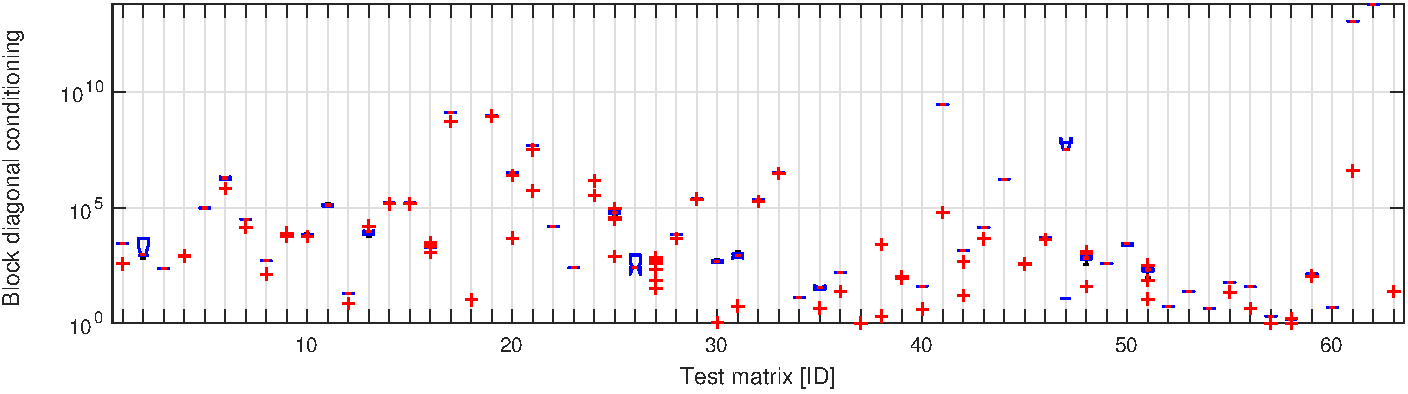
\includegraphics[width=\textwidth]{plots/boxplot_log_cond}
\caption
[Boxplot for the distribution of the condition numbers]
{Boxplot for the distribution of the condition numbers 
         of the diagonal blocks ($\kappa_1(D_i)$) using supervariable 
         agglomeration with the block size set to 24. For each matrix, the blue 
         central box shows where most of the condition numbers are located, the 
         red crosses indicate outliers.}
\label{2017-adaptive-block-jacobi:fig:blockcondnums}
\end{center}
\end{figure}

\subsection{Reduced precision preconditioning}

In the first experiment, we investigate how a reckless/adaptive reduction of the
precision for the representation of the block-Jacobi preconditioner impacts the
convergence rate of the PCG iterative solver. By recklessly reducing the
precision format used for storing the block-diagonal inverse, essential
information may be lost, which slows down the convergence of the
iterative solver. In the worst case, the diagonal blocks may become singular, or
the entries may fall outside of the data range that can be represented in the
chosen precision; both cases would likely result in the algorithm's breakdown. 
We
emphasize that the distinct preconditioners only differ in the format that is
leveraged to store the block inverse. Conversely, the problem-specific diagonal
block pattern is not affected, and
all computations are realized in \fpd.

The three leftmost columns in the right part of Table~\ref{2017-adaptive-block-jacobi:tab:matrices} report
the iterations required for convergence of  the PCG method when storing the
block-inverse preconditioner in \fpd, \fps, or \fph. We observe
that storing the preconditioner in \fps usually has only a mild impact on the
preconditioner quality. In most cases, the PCG iteration count matches the one
where the preconditioner is stored in \fpd. In a few cases, the PCG converges
even faster when storing the preconditioner in \fps. Conversely, if
the preconditioner is stored in \fph, the PCG does not converge in
most cases. Therefore, \fph storage cannot be recommended as the
default choice. In the right-most column of Table~\ref{2017-adaptive-block-jacobi:tab:matrices}, we
report the iteration count for the PCG method preconditioned with \apbj. We
observe that, except for some noise, the \apbj preserves the quality of the
preconditioner and the convergence rate of the \fpd solver.
Figure~\ref{2017-adaptive-block-jacobi:fig:blockinfo} shows that most of the time the adaptively
chosen precision is single or half precision, with relatively few instances
o of double.

\subsection{Energy model}

Having validated that the \apbj preconditioner preserves the convergence rate of
the iterative solver, we next quantify the advantage of the adaptive precision
block-Jacobi over a standard block-Jacobi using double precision. For this
purpose, we specifically focus on the  energy efficiency, as this has been
identified as an important metric (on par with performance) for future exascale
systems.

In terms of energy consumption, the accesses to main memory (MEMOPS)
are at least an order
of magnitude more expensive than FLOPs, and this gap is
expected to increase in future systems~\cite{shalf}.
For this reason, in the energy model, we ignore the arithmetic operations
(including the access to the data in the processor registers as well as caches)
and consider the data transfers from main memory only. Our energy model for
estimating the global energy consumption of the solver builds on the premise
that the energy cost of memory accesses is linearly dependent on the bit length
of the data.

Furthermore, as we only aim to estimate the energy efficiency of the \apbj
preconditioner \textit{relative} to the standard \fpd block-Jacobi
preconditioner, we will set the (normalized) energy cost of accessing a single
bit of data as $1$ (energy-unit). The precision formats we consider employ 64, 
32,
and 16 bits.

For a problem of size $n$ with $n_z$ nonzero elements, the PCG method presented
in Section~\ref{2017-adaptive-block-jacobi:sec:cg} and preconditioned with a block-Jacobi preconditioner
(consisting of $N$ diagonal blocks of dimensions $m_1\times m_1,\ldots,m_N\times
m_n$) performs:
\begin{equation}
\label{2017-adaptive-block-jacobi:eqn:cost}
\underbrace{14 n \cdot \fpd}_\mathrm{vector\ memory\ transfers} + 
\underbrace{(2 n + n_z) \cdot \fpd + (n+n_z)\cdot \inti}_\mathrm{CSR-SpMV\ 
memory\ transfers} +
\underbrace{2 n \cdot \fpd +
\sum_{i=1}^{N} m_i^2 \cdot \fpv_i
}_\mathrm{preconditioner\ memory\ transfers}
\end{equation}
data transfers (from memory) per iteration, where $\fpv_i$ denotes the precision
format selected for the $i$-th diagonal block of the preconditioner. The data
transfer volume of the block-Jacobi preconditioner thus depends on the format
employed to store the block inverse. For example, with the PCG running in \fpd, 
the approach also employs \fpd to maintain the
block-Jacobi preconditioner. Further, we also consider variants that store
the preconditioner entirely in \fps or \fph and a more sophisticated
strategy that adapts the format of the distinct preconditioner blocks to the
data.

\begin{figure}[t]
\begin{center}
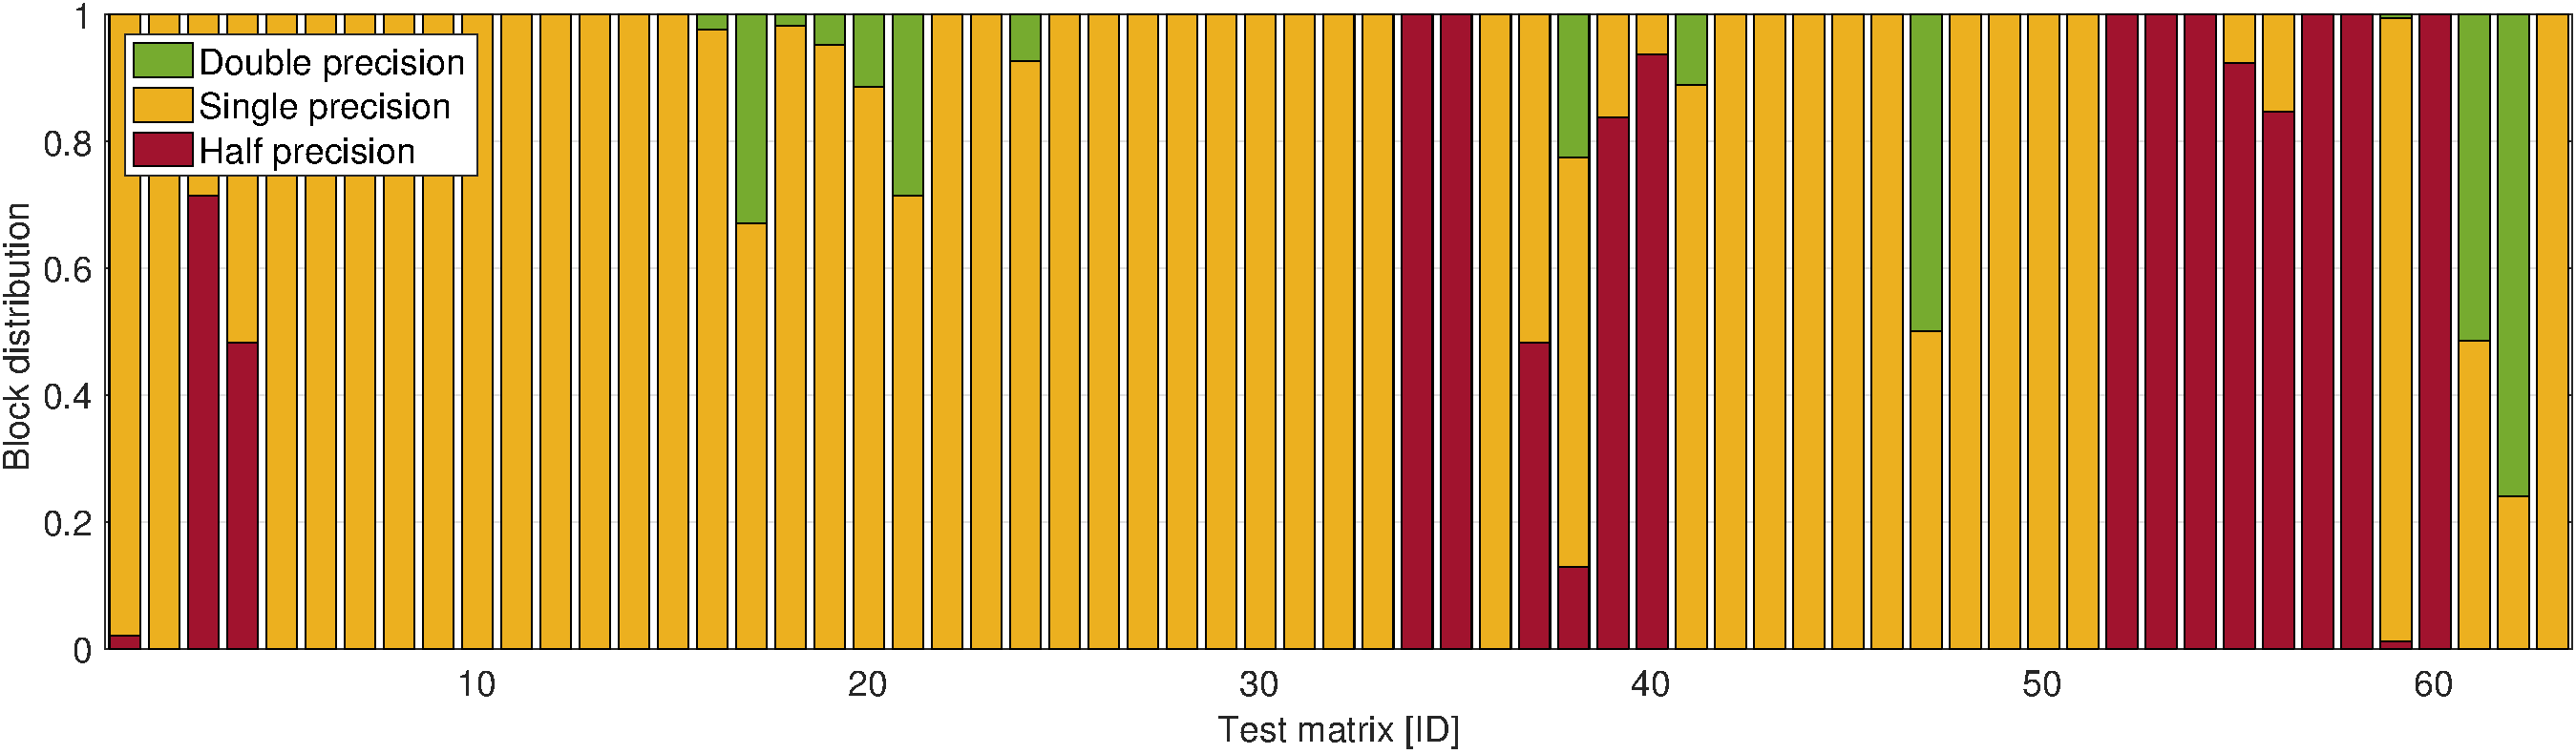
\includegraphics[width=\textwidth]{plots/blockinfo_adapt}
\caption
[Breakdown of the diagonal blocks stored in \fpd, \fps, or \fph.]
{Details on the adaptive precision block-Jacobi. Breakdown of the 
diagonal blocks stored in \fpd, \fps, or \fph.}
\label{2017-adaptive-block-jacobi:fig:blockinfo}
\end{center}
\end{figure}

\begin{figure}[t]
\begin{center}
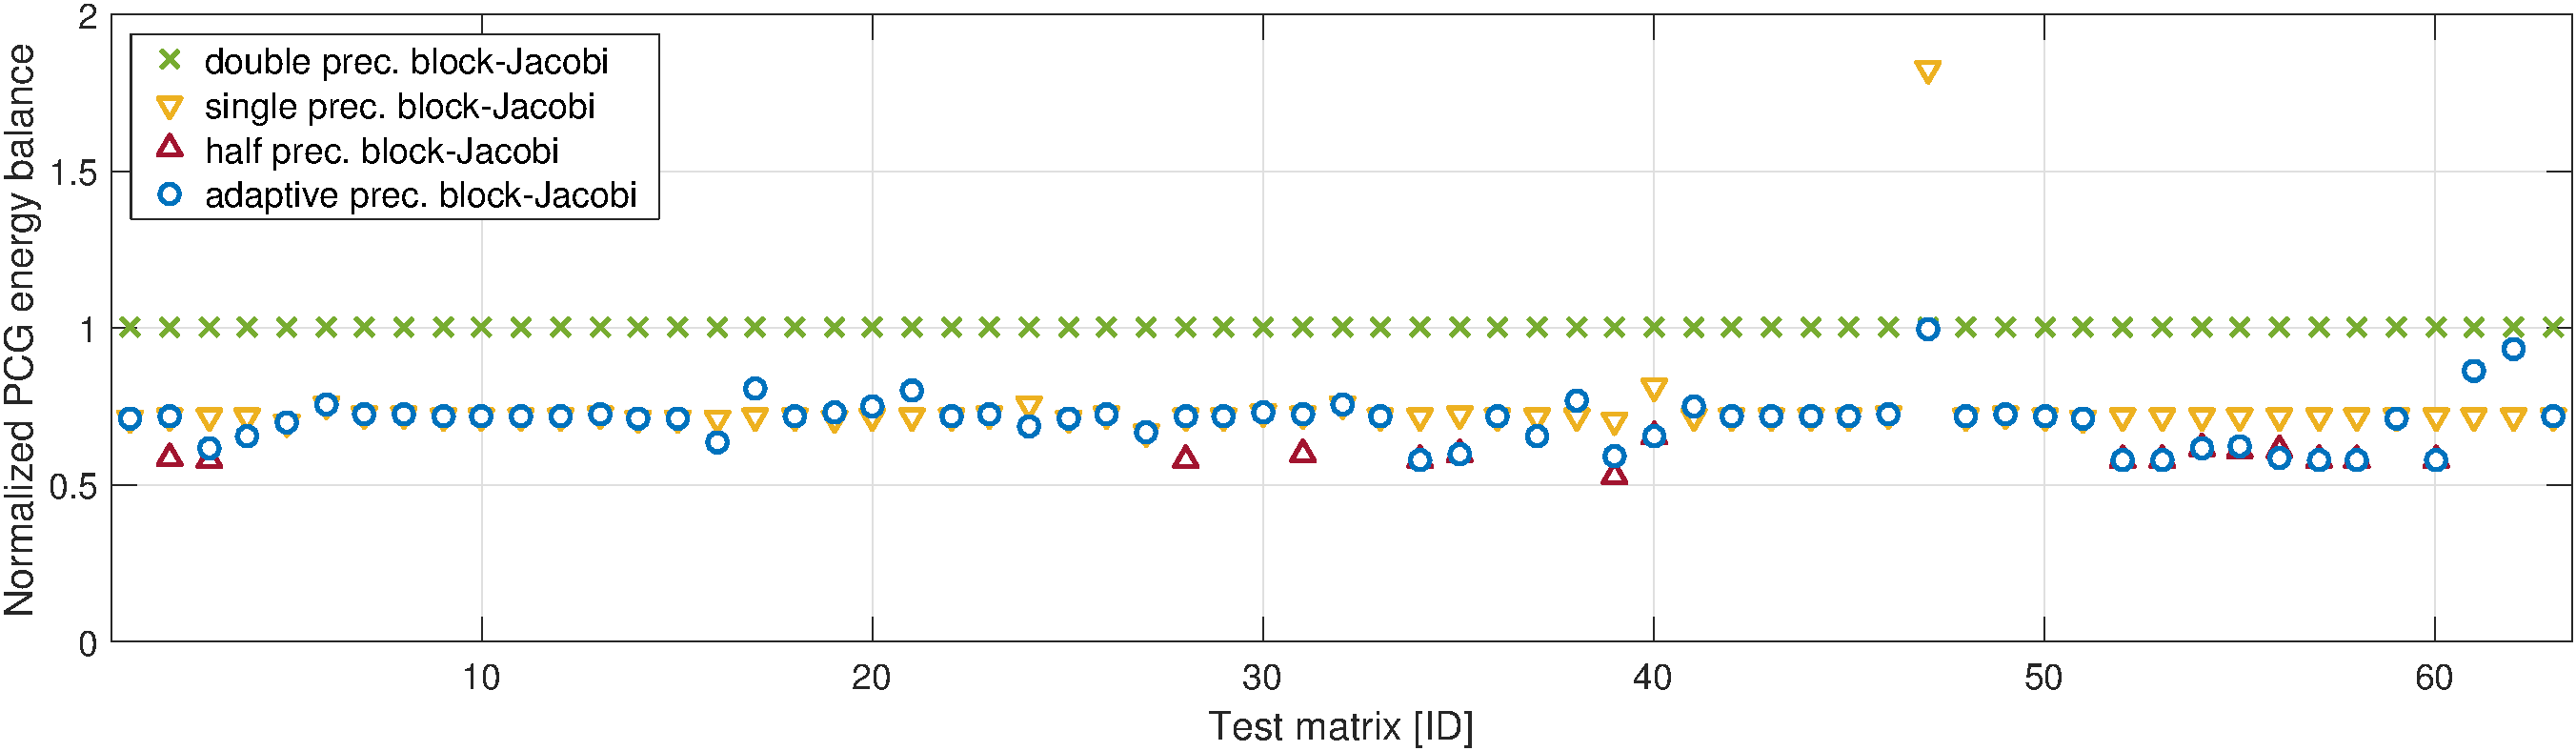
\includegraphics[width=\textwidth]{plots/fcg_energy_rel_adapt}
\caption
[Energy efficiency of PCG with block-Jacobi using various precisions]
{Energy efficiency analysis of the PCG with block-Jacobi preconditioning
	using different floating point formats for storing the preconditioner. The
	energy cost of all methods is normalized to the energy cost of the standard
	implementation using \fpd for storing the block-Jacobi preconditioner.}
\label{2017-adaptive-block-jacobi:fig:energyanalysis}
\end{center}
\end{figure}

For the \apbj approach, we visualize  the use of \fpd, \fps, and \fph for 
storing the diagonal blocks (Figure~\ref{2017-adaptive-block-jacobi:fig:blockinfo}). Comparing this 
information
with the data in Figure~\ref{2017-adaptive-block-jacobi:fig:blockcondnums}, we can identify a relationship
between the conditioning of the blocks and the storage precision format: \fpd 
is primarily employed for those cases comprising very ill-conditioned
blocks. Furthermore, the information in Figure~\ref{2017-adaptive-block-jacobi:fig:blockinfo} also
shows the savings that can be attained in terms of (1) memory usage
to store the preconditioner and (2) data transfers per iteration to retrieve 
data from main memory. However, note that these savings do not take into
account the total cost of the PCG method but only those costs strictly 
associated
with the preconditioner application. 
Furthermore, the data in Figure~\ref{2017-adaptive-block-jacobi:fig:blockinfo} does not reflect the
potentially slower convergence caused by using reduced precision storage.

To avoid the previous two pitfalls, in our final experiment we compute the total
data transfers of a single iteration of the PCG method with the block-Jacobi
preconditioner stored in \fpd, \fps, \fph, or adaptive precision, 
see equation~(\ref{2017-adaptive-block-jacobi:eqn:cost}). To obtain an estimated total data transfer 
volume,
we then combine the data transfer volume per iteration with the number of
iterations needed to reach convergence in each case---ignoring those cases for
which half precision does not converge.

In Figure~\ref{2017-adaptive-block-jacobi:fig:energyanalysis}, we show the total energy balance
\textit{relative} to the standard approach that maintains the block-Jacobi
preconditioner in double precision.

Some key observations from this last experiment are listed below.
\begin{itemize}
\item Storing the block-Jacobi preconditioner in \fps often reduces the
total energy cost. However, for those cases where the information loss increases
the PCG iteration count, storing the preconditioner in \fps can have a
negative impact on the energy balance.
\item For the (few) cases where the block-inverse matrix can be stored in
\fph without the PCG losing convergence, the total energy cost can be
decreased by up to 50\%.
\item Using the \apbj preconditioner never increases the total energy 
consumption. 
\item In most cases, the \apbj preconditioner matches or outperforms the
efficiency of storing the preconditioner in \fps. If the problem
characteristics allow for it, the \apbj preconditioner employs \fph to
match the half precision efficiency while maintaining convergence for the other
cases.
\item The \apbj preconditioner ``automatically'' detects the need to store a
diagonal block in \fpd to avoid convergence degradation.
\end{itemize}

Finally, we note that, for memory bandwidth-bound operations like the 
block-Jacobi
preconditioned CG considered here, the performance is largely determined by the
data transfer volume. Therefore, the results shown in 
Figure~\ref{2017-adaptive-block-jacobi:fig:energyanalysis}
and the insights gained from that experiment carry over to the runtime
performance of the adaptive precision block-Jacobi preconditioner. In summary,
these experiments prove that the \apbj preconditioner is an efficient strategy
for improving the resource usage, energy consumption, and runtime performance of
iterative solvers for sparse linear systems.

